\documentclass[defaultstyle,12pt]{report}
\usepackage[utf8]{inputenc}
\usepackage{graphicx}
\usepackage{hyperref}
\usepackage {wrapfig}

\hypersetup{ colorlinks=false,
			citecolor=red,
			breaklinks=true,
			bookmarks=true,
			bookmarksnumbered=true,
			bookmarksopen=true,
			pdftitle={Projecto do Oscilador de Fermi}, % EDIT THIS LINE
			pdfauthor={Filipe Duarte, Filipe Novais},
			pdfsubject={THE SUBJECT}, % EDIT THIS LINE
			pdfcreator={LaTeX with TeXmaker},
			pdfkeywords={} % EDIT THIS LINE
}

\begin{document}


\title{Projecto do oscilador de Fermi}
\maketitle

\section{Introdução}

Consideremos o seguinte sistema oscilante: uma partícula de massa m, é deixada cair desde uma altura h, sobre uma plataforma de massa M unida a um mola elástica de constante k. A partícula cai e choca elasticamente com a plataforma, o bloco sobe e desce, a plataforma oscila e voltam a se encontrar ao cabo de um certo tempo, chocam e assim, sucessivamente.\\

Aplicamos a segunda lei de Newton para estudar o movimento do sistema formado pela mola e a plataforma, e as equações do movimento de queda livre para estudar o movimento do bloco. No momento do choque, aplicamos o princípio de conservação do momento linear e da energia.

O sistema é conservativo, a energia do sistema formado pelo bloco, a mola e a plataforma é mantida constante.

\section{Modo de operar com o programa}

Todas os 10 botões do programa são muito simples de executar.

Os 5 primeiros, são usados para podemos definir todas as variaveis que existe no programa. Todas elas tem um valor minimo e um valor maximo.



\begin{figure}[!htb]
\begin{center}
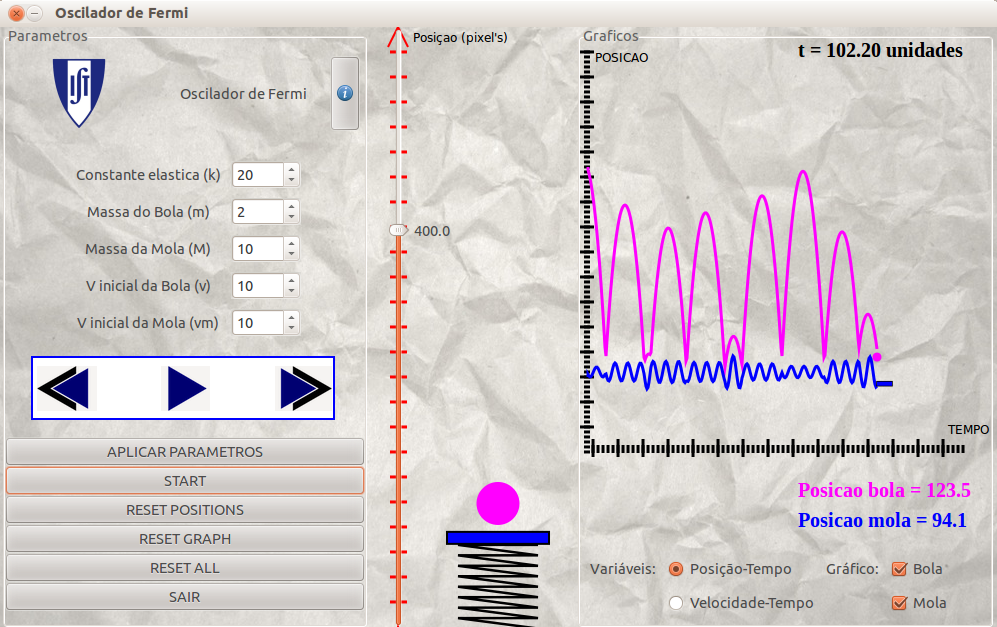
\includegraphics[scale=0.33]{programa.png}\\\
\end{center}
\end{figure}

 Elas são:

\begin{center}
    \begin{tabular}{ | l | l | l | p{4cm} |}
    \hline
    Grandezas & Valor minimo & Valor maximo & Comentário \\ \hline
    Constante de elastica & 0 & 10000 & Esta K é sempre positiva. O seu valor inicial e de  20\\ \hline
    Massa da bola & 1 & 100 & A M assume sempre valores positivos. O seu valor inicial e de 2.
   \\ \hline
    Massa da mola & 1 & 100 & A M da mola assume sempre valores positivos. O seu valor inicial e de 10. \\
    \hline
    Velocidade Inicial da bola & 0 & 100 & A V inicial da bola apenas foi defenida no sentido do oscilador, por isso não assume valores negativos.  seu valor inicial e de 10. \\
    \hline
    Velocidade Inicial da Mola & 0 & 100 & A V inicial da mola apenas foi defenida no sentido do oscilador, por isso não assume valores negativos. E o seu valor inicial e de 10 \\
    \hline
    \end{tabular}
    \\
   
    
   
    Os ultimos 5 botoes dos programas são os utilizados para comandar o programa.\\

   
   
    
    \begin{center}
    \begin{tabular}{ | l | p{5cm} |}
    \hline
    Controladores & definição \\ \hline
    Aplicar Parametros & O aplicar parametros serve para depois de mudar os parametros, aplicar as mudanças á simulaçao \\ \hline
    Star and Stop & O controlador star and stop e utilizado para começar e parar o programa. \\ \hline
    Reset Positions & Serve apenas para meter os objectos nas posiçoes iniciais e manter todos os parametros \\ \hline
    Reset Graph & Serve para limpar o grafico existente e escrever um grafico novo\\ \hline    
    Reset All & Serve para meter, tanto os parametros como as posiçoes da bola e da mola, nas condiçoes iniciais \\ \hline
    Sair & Serve para chamar uma janela que permite o fecho do programa  \\ \hline
   
    \end{tabular}
\end{center}
    
\end{center}

  \begin{center}
    \begin{tabular}{ | l | p{5cm} |}
    \hline
    Controlar Tempo & Funçao \\ \hline
    Slow, Fast e Play & Estas eventboxs servem para diminuir, aumentar ou manter o tempo inicial, durante o decorrer do programa \\\hline
  
    \end{tabular}
   
\end{center}
    
    \pagebreak

\section{Graficos}
  
- Do nosso lado direito do programa podemos observar o desenvolvimento da posição ao longo do tempo experiência que fazemos\\

- Podemos escolher a opcao de ver um ou dois graficos, o da bola e/ou o da mola, atraves das checkboxs no canto inferior direito. 
\\\\\\\




\begin{figure}[!htb]
\begin{center}
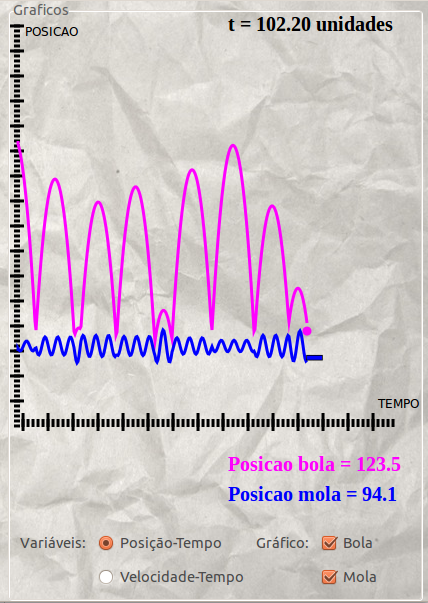
\includegraphics[scale=0.45]{grafico1.png}
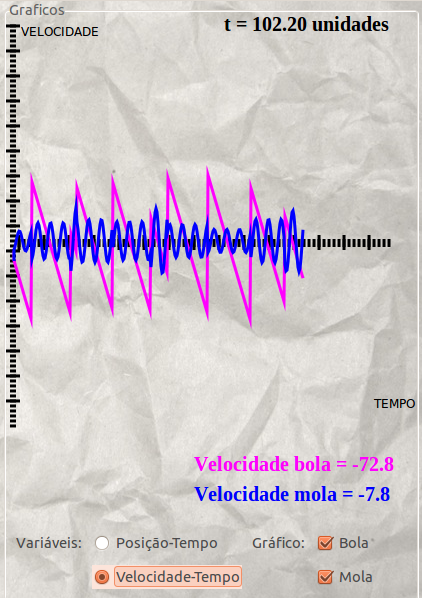
\includegraphics[scale=0.45]{grafico2.png}
\end{center}
\end{figure}


\end{document}
